\documentclass{article}
\usepackage[top=0.5in, bottom=0.5in, left=1in, right=1in]{geometry}
\usepackage{graphicx}
\usepackage{listings}
% Configure listings
\usepackage{color}
\lstset{% setup listings
  language=R,% set programming language
  basicstyle=\small\ttfamily,% basic font style
  keywordstyle=\color{blue},% keyword style
  commentstyle=\ttfamily\itshape,% comment style
  numbers=left,% display line numbers on the left side
  numberstyle=\scriptsize,% use small line numbers
  numbersep=10pt,% space between line numbers and code
  tabsize=3,% sizes of tabs
  showstringspaces=false,% do not replace spaces in strings by a certain character
  captionpos=b,% positioning of the caption below
  breaklines=true,% automatic line breaking
  escapeinside={(*}{*)},% escaping to LaTeX
  extendedchars=false,% prohibit extended chars (chars of codes 128--255)
  literate={"}{{\texttt{"}}}1{<-}{{$\leftarrow$}}1{<<-}{{$\twoheadleftarrow$}}1
  {~}{{$\sim$}}1{<=}{{$\le$}}1{>=}{{$\ge$}}1{!=}{{$\neq$}}1{^}{{$^\wedge$}}1,% item to replace, text, length of chars
  alsoletter={.<-},% becomes a letter
  alsoother={$},% becomes other
  otherkeywords={
    !=, ~, $, *, \&, \%/\%, \%*\%, \%\%, <-, <<-, /, \%>\%,
    select_if, is.numeric, NA
  },% other keywords
  deletekeywords={c, length}% remove keywords
}

\begin{document}

% --------------------------------------------------
\section{Directions}
% --------------------------------------------------
Please follow the following directions:

\begin{enumerate}
\item Read Section \ref{sec:summary} (Summary) by yourself; try to answer the
  questions on your own
\item When prompted, discuss all Sections with your small group
\item When prompted, join in the full-group discussion
\end{enumerate}

% --------------------------------------------------
\section{Summary} \label{sec:summary}
% --------------------------------------------------
Take a look at the following code output, and try to 'get a sense' of the autos
data. Note that we haven't discussed all the concepts below! Try, to the best of
your ability, to answer the following questions:

\begin{enumerate}
\item What do 'Min.', '1st Qu.', 'Median', "Mean", '3rd Qu.', and 'Max.' mean?
\item Which variable has the most NA's?
\item For which variables do 'Mean' and 'Median' disagree?
\end{enumerate}

\begin{lstlisting}
> df_autos %>% select_if(is.numeric) %>% summary
   symboling       normalized_losses  num_of_doors     wheel_base
 Min.   :-2.0000   Min.   : 65       Min.   :2.000   Min.   : 86.60
 1st Qu.: 0.0000   1st Qu.: 94       1st Qu.:2.000   1st Qu.: 94.50
 Median : 1.0000   Median :115       Median :4.000   Median : 97.00
 Mean   : 0.8341   Mean   :122       Mean   :3.123   Mean   : 98.76
 3rd Qu.: 2.0000   3rd Qu.:150       3rd Qu.:4.000   3rd Qu.:102.40
 Max.   : 3.0000   Max.   :256       Max.   :4.000   Max.   :120.90
                   NA's   :41        NA's   :2
     length          width           height       curb_weight
 Min.   :141.1   Min.   :60.30   Min.   :47.80   Min.   :1488
 1st Qu.:166.3   1st Qu.:64.10   1st Qu.:52.00   1st Qu.:2145
 Median :173.2   Median :65.50   Median :54.10   Median :2414
 Mean   :174.0   Mean   :65.91   Mean   :53.72   Mean   :2556
 3rd Qu.:183.1   3rd Qu.:66.90   3rd Qu.:55.50   3rd Qu.:2935
 Max.   :208.1   Max.   :72.30   Max.   :59.80   Max.   :4066

 num_of_cylinders  engine_size         bore          stroke
 Min.   : 2.00    Min.   : 61.0   Min.   :2.54   Min.   :2.070
 1st Qu.: 4.00    1st Qu.: 97.0   1st Qu.:3.15   1st Qu.:3.110
 Median : 4.00    Median :120.0   Median :3.31   Median :3.290
 Mean   : 4.38    Mean   :126.9   Mean   :3.33   Mean   :3.255
 3rd Qu.: 4.00    3rd Qu.:141.0   3rd Qu.:3.59   3rd Qu.:3.410
 Max.   :12.00    Max.   :326.0   Max.   :3.94   Max.   :4.170
                                  NA's   :4      NA's   :4
 compression_ratio   horsepower       peak_rpm       city_mpg
 Min.   : 7.00     Min.   : 48.0   Min.   :4150   Min.   :13.00
 1st Qu.: 8.60     1st Qu.: 70.0   1st Qu.:4800   1st Qu.:19.00
 Median : 9.00     Median : 95.0   Median :5200   Median :24.00
 Mean   :10.14     Mean   :104.3   Mean   :5125   Mean   :25.22
 3rd Qu.: 9.40     3rd Qu.:116.0   3rd Qu.:5500   3rd Qu.:30.00
 Max.   :23.00     Max.   :288.0   Max.   :6600   Max.   :49.00
                   NA's   :2       NA's   :2
  highway_mpg        price
 Min.   :16.00   Min.   : 5118
 1st Qu.:25.00   1st Qu.: 7775
 Median :30.00   Median :10295
 Mean   :30.75   Mean   :13207
 3rd Qu.:34.00   3rd Qu.:16500
 Max.   :54.00   Max.   :45400
                 NA's   :4
\end{lstlisting}

\newpage
% --------------------------------------------------
\section{Graphic}
% --------------------------------------------------

Take a look at the following graphic, and answer the following questions:

\begin{enumerate}
\item What does Figure \ref{fig:mpg-vs-usd} imply about city vs highway driving?
  Why might this be?
\item What does Figure \ref{fig:mpg-vs-usd} imply about the relationship between
  fuel efficiency and price?
\item Notice that efficiency values tend to form horizontal 'stripes' -- why is
  this?
\end{enumerate}

\begin{figure}[!ht]
  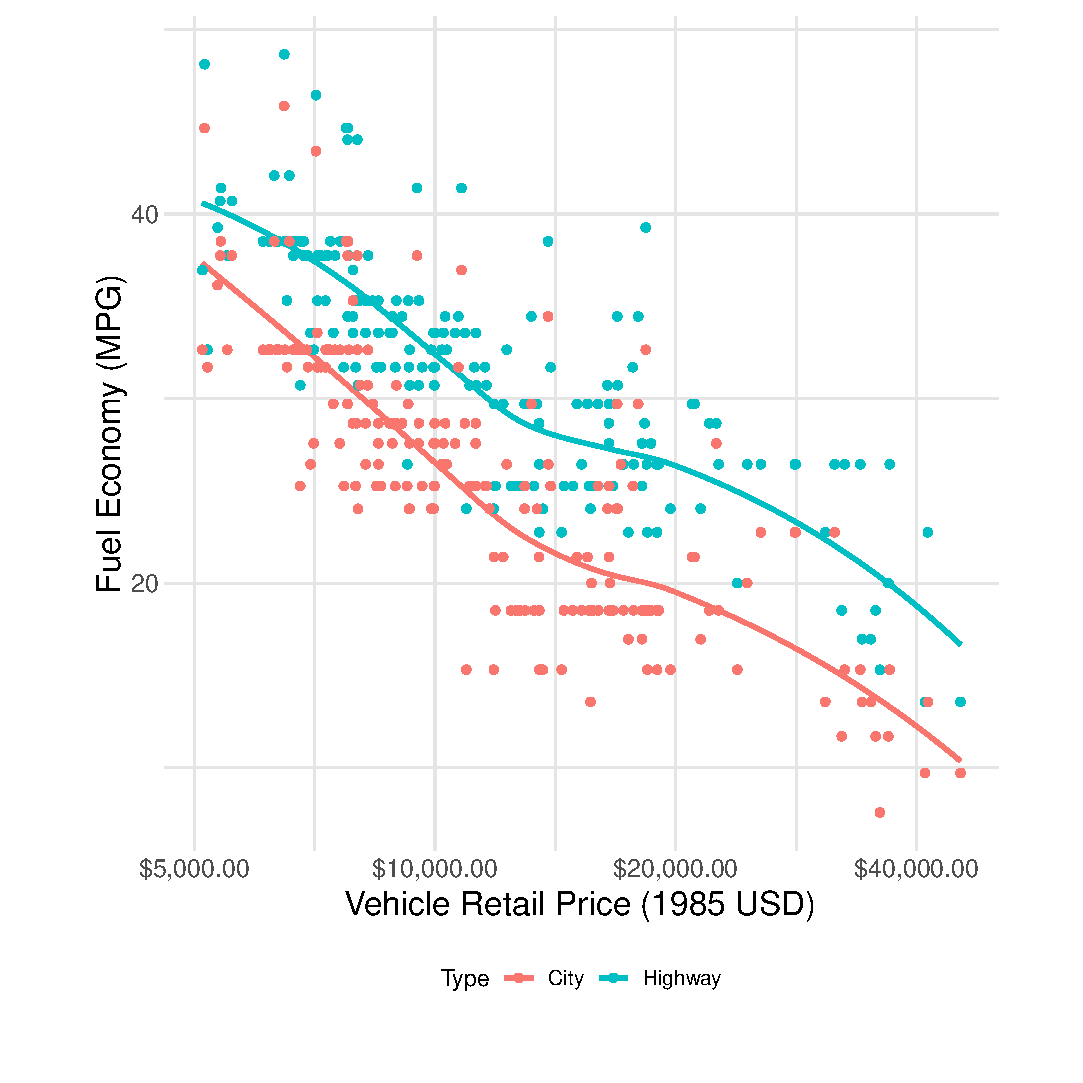
\includegraphics[width=0.90\textwidth]{../images/mpg_vs_usd}
  \caption{Vehicle efficiency vs price for the UCI autos dataset.}
  \label{fig:mpg-vs-usd}
\end{figure}

\end{document}
